% The entire content of this work (including the source code
% for TeX files and the generated PDF documents) by 
% Hongxiang Chen (nicknamed we.taper, or just Taper) is
% licensed under a 
% Creative Commons Attribution-NonCommercial-ShareAlike 4.0 
% International License (Link to the complete license text:
% http://creativecommons.org/licenses/by-nc-sa/4.0/).
\documentclass{article}

% My own physics package
% The following line load the package xparse with additional option to
% prevent the annoying warnings, which are caused by the package
% "physics" loaded in package "physicist-taper".
\usepackage[log-declarations=false]{xparse}
\usepackage{physicist-taper}
\makenomenclature % For an index of symbols.

\title{TR Invariant T.I.}
\date{\today}
\author{Taper}


\begin{document}


\maketitle
\abstract{
    An incomplete note of dissertation by Taylor Hughes
    \cite{Hughes2009}.
}
\tableofcontents
Start with chapter 2.

Questions:
\begin{itemize}
    \item Do we have a precise definition of \textit{topological phase
        transition}?
\end{itemize}

\section{Spectrum of \texorpdfstring{$(2+1)$}-d Lattice Dirac Model}
\label{sec:2+1d-LDirac Model}
\begin{align}
    H_{LD} &= \sum_{m,n}\left\{
        i \left[ c^\dagger_{m+1,n}\sigma^x c_{m,n}
            - c^\dagger_{m,n}\sigma^x c_{m+1,n}\right]
        + i \left[ c^\dagger_{m,n+1}\sigma^y c_{m,n}
            - c^\dagger_{m,n}\sigma^y c_{m,n+1} \right]
        \right.
        \nonumber\\
        &- \left[
            c^\dagger_{m+1,n}\sigma^z c_{m,n}
            + c^\dagger_{m,n}\sigma^z c_{m+1,n}
            + c^\dagger_{m,n+1}\sigma^z c_{m,n}
            + c^\dagger_{m,n}\sigma^z c_{m,n+1}
        \right]
        \nonumber\\
        & \left. + (2-m) c^\dagger_{m,n}\sigma^z c_{m,n}
        \vphantom{xx}\frac\hbar2
    \right\}
\end{align}

Above is the lattice model (eq.2.19) of \cite{Hughes2009}. Here it
should be noted that $c_{m,n}=(c_{u,m,n}, c_{v,m,n})$ for two degrees
of freedom. 

This Hamiltonian is solved here with a infinite cylinder geometry, i.e.
the lattice is infinite in $x$ direction while being periodic in $y$
direction. Because of this special setup, the $p_x$ is still a good
quantum number. Therefore we can do a fourier expansion in $x$
direction:

\begin{equation}
    c_{m,n} = \frac{1}{\sqrt{L_x}} \sum_{p_x} e^{ip_x m} c_{p_x,n}
\end{equation}

The resulted Hamiltonian is 

\begin{align}
    \tilde H_{LD} = \sum_{n,p_x}\quad &
    2\sin(p_x) c^\dagger_{p_x,n}\sigma^x c_{p_x,n}
    +i \left[ c^\dagger_{p_x,n+1}\sigma^y c_{p_x,n} - 
        c^\dagger_{p_x,n+1}\sigma^y c_{p_x,n}\right]
    \nonumber\\
    &- \left[ 2\cos(p_x) c^\dagger_{p_x,n}\sigma^z c_{p_x,n}
        c^\dagger_{p_x,n+1}\sigma^z c_{p_x,n}
        + c^\dagger_{p_x,n}\sigma^z c_{p_x,n+1}
    \right]
    \nonumber\\
    &+ (2-m) c^\dagger_{p_x,n}\sigma^z c_{p_x,n}
\end{align}

This Hamiltonian can be solved by acting it on the test wavefunction:
\begin{equation}
    \ket{\psi_{p_x}} = \sum_n \psi_{p_x,n,u} c^\dagger_{p_x,n,u} +
                        \psi_{p_x,n,v} c^\dagger_{p_x,n,v} \ket{0}
\end{equation}

Note, in choosing the test wavefunction, $u$ and $v$ could not be
seperated, because there is still interaction between the two
component in terms like $c^\dagger_{p_x,n}\sigma^x c_{p_x,n}$.
If we calculate $\tilde H_{LD}\ket{\psi_{p_x}} = E_{p_x}
\ket{\psi_{p_x}}$, we would get after careful calculation:

\begin{align}
    & \sum_n
    c^\dagger_{p_x,n} A   \psi_{p_x,n-1}
    + c^\dagger_{p_x,n} B \psi_{p_x,n} 
    + c^\dagger_{p_x,n} C \psi_{p_x,n+1}
    \nonumber\\
    &= E_{p_x} \sum_n c^\dagger_{p_x,n}\psi_{p_x,n}
\end{align}
where
\begin{align}
    c^\dagger_{p_x,n} &= \begin{pmatrix}
        c^\dagger_{p_x,n,u},  c^\dagger_{p_x,n,v}
    \end{pmatrix} \\
    A &= i\sigma^y - \sigma^z \\
    B &= 2\sin(p_x)\sigma^x - 2\cos(p_x)\sigma^z + (2-m)\sigma^z \\
    C &= -i\sigma^y - \sigma^z \\
    \psi_{p_x,n} &= \begin{pmatrix}
        \psi_{p_x,n,u} \\ \psi_{p_x,n,v}
    \end{pmatrix}
\end{align}

Suppose there is $N$ lattice in the $y$ direction. Then the periodic
boundary condition implies that $\psi_{N+1}=\psi_{n=1}$, and
$\psi_{n=0} = \psi_N$.

Therefore, the eigenvalue equation could be turned into a matrix form:
\begin{align}
    H_{\text{disc}} \psi \equiv 
    \begin{pmatrix}
        B   & C &        &   & A \\
        A   & B & C      &   & \\
            & A & B      & C & \\
            &   & \cdots &   & \\
            &   & A      & B & C \\
        C   &   &        & A & B
    \end{pmatrix}
    \begin{pmatrix}
        \psi_{p_x,1} \\
        \psi_{p_x,2} \\
        \cdots \\
        \\
        \\
        \psi_{p_x,N} \\
    \end{pmatrix} =
    E_{p_x}
    \begin{pmatrix}
        \psi_{p_x,1} \\
        \psi_{p_x,2} \\
        \cdots \\
        \\
        \\
        \psi_{p_x,N} \\
    \end{pmatrix}
\end{align}

    \subsection{Numerical result}
    \label{sec:Numerical result}
    \textbf{Note}: Results in this section are contained in the file
    "Lattice Dirac Model (2+1)-d.nb", and the file
    "Dirac\_Lattice\_Model\_21\_d.m".

    Let us take $N=3$ for simplicity. The eigenvalue problem is solve
    using Mathematica, and the $6$ eigenvalues are:
    \begin{equation}
        \begin{pmatrix}
        -\sqrt{m^2+4 m \cos (\text{px})+4}\\
        \sqrt{m^2+4 m \cos (\text{px})+4}\\
        -\sqrt{m^2+4 m \cos (\text{px})-6 m-12 \cos (\text{px})+16}\\
        -\sqrt{m^2+4 m \cos (\text{px})-6 m-12 \cos (\text{px})+16}\\
        \sqrt{m^2+4 m \cos (\text{px})-6 m-12 \cos (\text{px})+16}\\
        \sqrt{m^2+4 m \cos (\text{px})-6 m-12 \cos (\text{px})+16}
        \end{pmatrix}
    \end{equation}

    It is found that at $m=-2$, there is a band crossing at $p_x=0$:
    \begin{figure}[H]
        \centering
        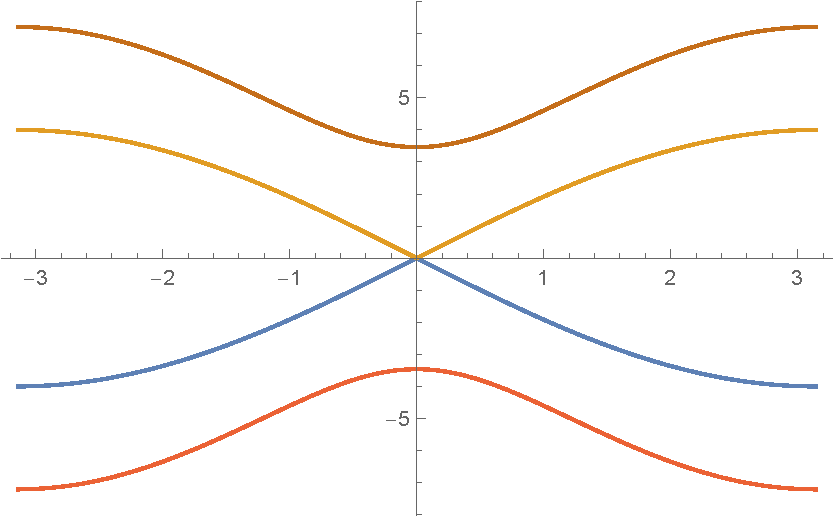
\includegraphics[width=0.6\linewidth]{pics/N6m-2.pdf}
        \caption{The Eigenvalue plot for $m=-2$. Plotted as
        $E_{p_x}$v $p_x$ }
    \end{figure}

    Also, at $m=2$, there is a band crossing at $p=\pm\pi$:
    \begin{figure}[H]
        \centering
        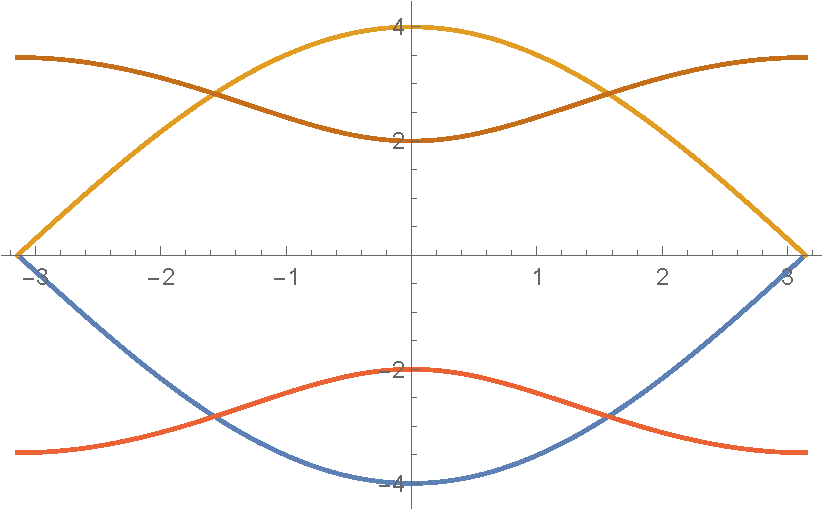
\includegraphics[width=0.6\linewidth]{pics/N6m2.pdf}
        \caption{The Eigenvalue plot for $m=2$. Plotted as
        $E_{p_x}$v$p_x$ }
    \end{figure}

    Since the paper will be focusing in points around $p_x=0$, I will
    focus in $m=-2$. In this case, I want to find more information
    about the eigenvectors. 
    
    When I looked blindly at the value $(m,p_x)=(-2,0)$, the
    Mathematica gave me two eigenvectors both corresponds to the
    eigenvalue $0$:
    \begin{equation}
        \{0,1,0,1,0,1\},\{1,0,1,0,1,0\}
    \end{equation}
    It led me to believe that there are two spin waves, with made with
    purely spin up waves and another of purely spin down waves. But
    this is not correct. 

    It is found later that the matrix $H_\text{disc}$ is singular
    (with determinant $0$) when $(m,p_x)=(-2,0)$. Also, a Matlab
    calculation shows that the eigenvectors of the crossing bands
    actually flunctuate between $\pm 1$ in a way illustrated as below:
    \begin{figure}[H]
        \centering
        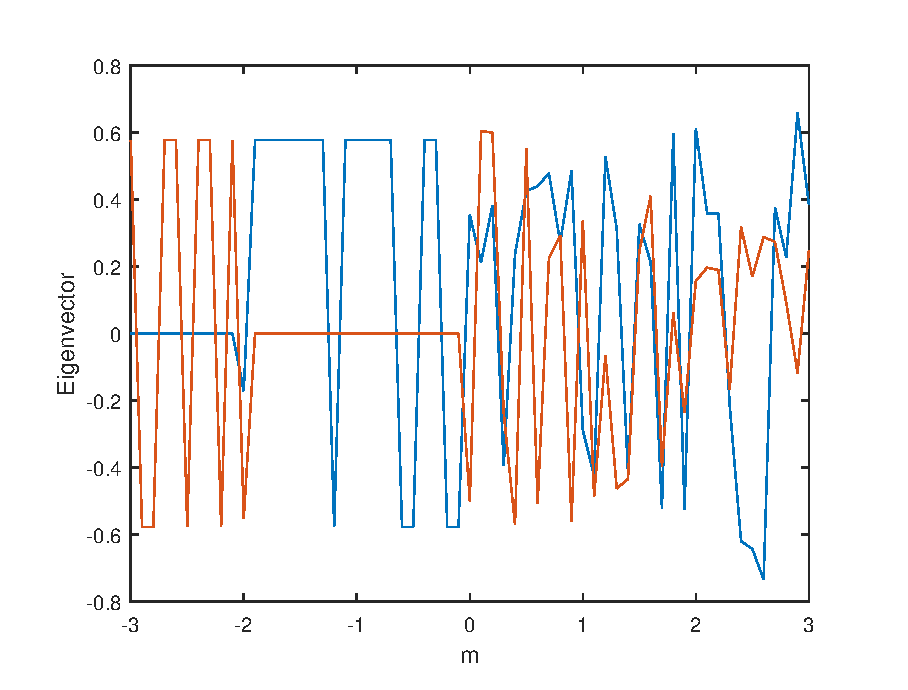
\includegraphics[width=0.6\linewidth]{pics/Eigenvector-m.eps}
    \end{figure}

    Also, the Mathematica solved eigenvector also demonstrate a
    drastical change around $m=-2$. For example, one component, when
    plotted against $p_x$ change from:
    \begin{figure}[H]
        \centering
        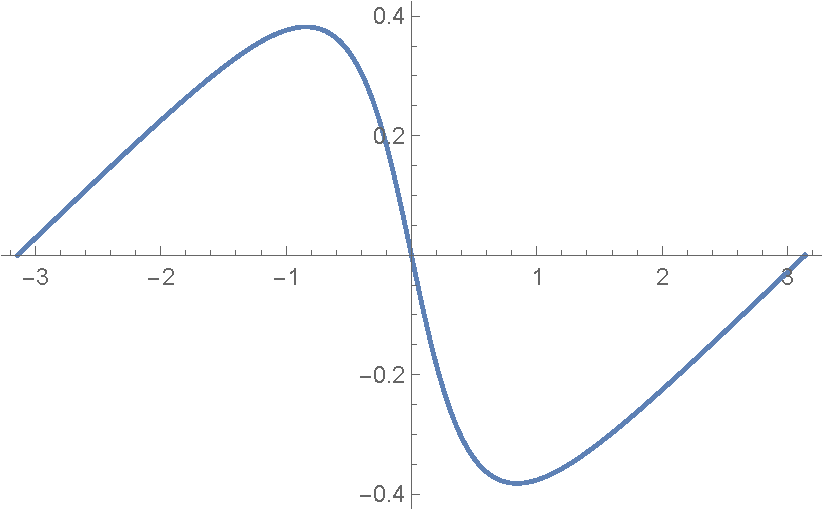
\includegraphics[width=0.6\linewidth]{pics/mN3.pdf}
        \caption{$m=-3$}
    \end{figure}
    to
    \begin{figure}[H]
        \centering
        \includegraphics[width=0.6\linewidth]{pics/{mN2.5}.pdf}
        \caption{$m=-2.5$}
    \end{figure}
    and suddenly to
    \begin{figure}[H]
        \centering
        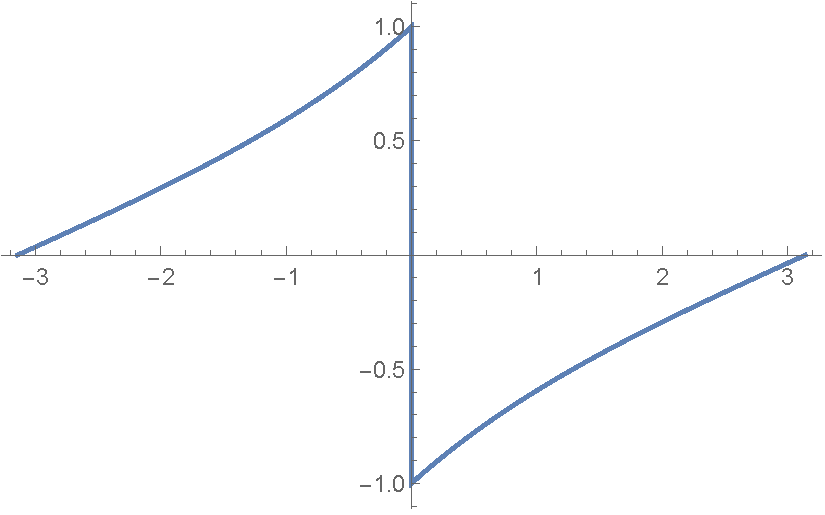
\includegraphics[width=0.6\linewidth]{pics/mN2.pdf}
        \caption{$m=-2$. There is a discontinuity at $p_x=0$}
    \end{figure}
    Finaly, it becomes smooth again:
    \begin{figure}[H]
        \centering
        \includegraphics[width=0.6\linewidth]{pics/{mN1.5}.pdf}
        \caption{$m=-1.5$}
    \end{figure}
    The details can be explored in the Mathematica notebook.
    
    Also, the case of $N=4$ is also calculated in Mathematica.
    There are similarly two crossing happening at $(m,p_x)$ equals
    $(-2,0)$ and $(2,\pm\pi)$.

    \begin{figure}[H]
        \centering
        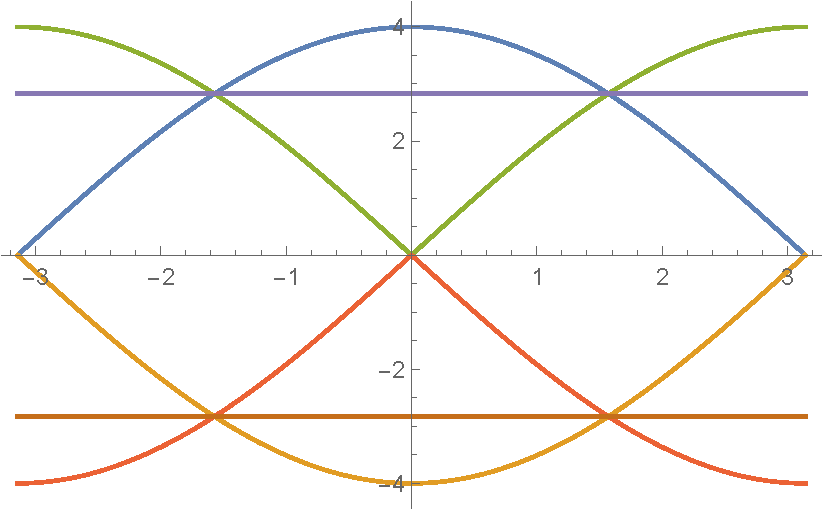
\includegraphics[width=0.6\linewidth]{pics/N8m2.pdf}
        \caption{$m=2$}
    \end{figure}
    \begin{figure}[H]
        \centering
        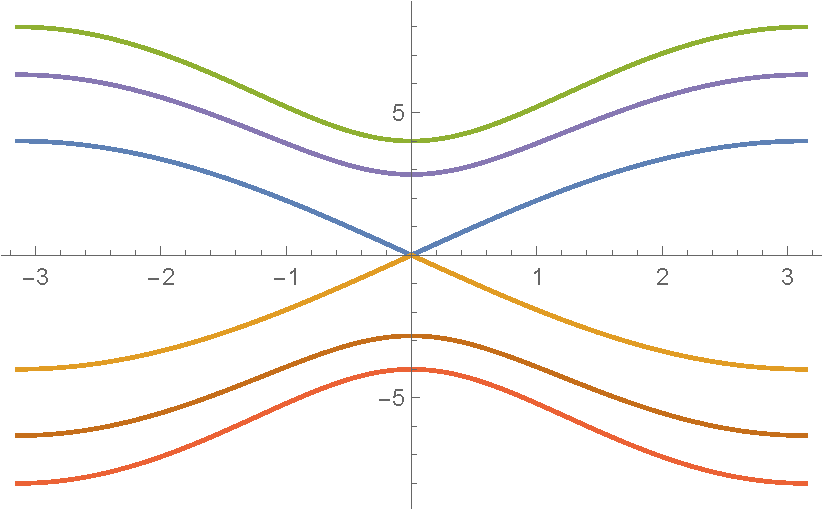
\includegraphics[width=0.6\linewidth]{pics/N8m-2.pdf}
        \caption{$m=-2$}
    \end{figure}

    Surprisingly, the two bands that cross are have exactly the same
    function dependence on $p_x$ and $m$ for the cases of $N=3$ and
    $N=4$.

    \subsection{Discussion about the Lattice Model}
    \label{sec:DisAboutLatticeModel}
    I notice that equation (2.19) transformed according to (2.20)
    is not exactly equation (2.21), but is:
    \begin{align}
        &H =\sum_{p_x,p_y} c^\dagger_{p_x,p_y}\times
        \nonumber\\
        &
        \left[
            2\sin(p_x)\sigma^x + 2\sin(p_y)\sigma^y
            +(2-m-2\cos(p_x)-2\cos(p_y))\sigma^z
        \right] c_{p_x,p_y}
    \end{align}
    This result does not become the continuum Dirac Hamiltonian as
    $p_x,p_y$ goes to zero. Therefore, I suspect that certain
    constants should be modified so that:

    \begin{align}
        H_{LD} &= \sum_{m,n}\left\{
            \frac{i}{2} \left[ c^\dagger_{m+1,n}\sigma^x c_{m,n}
                - c^\dagger_{m,n}\sigma^x c_{m+1,n}\right]
            + \frac{i}{2} \left[ c^\dagger_{m,n+1}\sigma^y c_{m,n}
                - c^\dagger_{m,n}\sigma^y c_{m,n+1} \right]
            \right.
            \nonumber\\
            &- \frac{1}{2}\left[
                c^\dagger_{m+1,n}\sigma^z c_{m,n}
                + c^\dagger_{m,n}\sigma^z c_{m+1,n}
                + c^\dagger_{m,n+1}\sigma^z c_{m,n}
                + c^\dagger_{m,n}\sigma^z c_{m,n+1}
            \right]
            \nonumber\\
            & \left. + (2-m) c^\dagger_{m,n}\sigma^z c_{m,n}
            \vphantom{\frac12}
        \right\}
    \end{align}

    This affects the numerical analysis effectively by the replacement
    $$\sigma^i \to \frac{1}{2}\sigma^i,\quad
        (2-m) \to 2(2-m) $$

    And the result is similar to previous study, except that the band
    crossing happens at different values of $m$. For example, the
    eigenvalue of original and the modified equation (2.21) are
    plotted in Mathematica notebook "Eq2.21-Demo.nb". Also, the
    solution to the infinite cylinder boundary condition has again two
    band crossings, each at $(m,p_x)$ equals $(0,0)$ and $(2,\pm\pi)$
    (for $N=3$ case).


\bibliography{cite}{}
\bibliographystyle{alphaurl}

\printnomenclature
\section{License}
The entire content of this work (including the source code
for TeX files and the generated PDF documents) by 
Hongxiang Chen (nicknamed we.taper, or just Taper) is
licensed under a 
\href{http://creativecommons.org/licenses/by-nc-sa/4.0/}{Creative 
Commons Attribution-NonCommercial-ShareAlike 4.0 International 
License}. Permissions beyond the scope of this 
license may be available at \url{mailto:we.taper[at]gmail[dot]com}.
\end{document}
